% Options for packages loaded elsewhere
\PassOptionsToPackage{unicode}{hyperref}
\PassOptionsToPackage{hyphens}{url}
%
\documentclass[
]{book}
\usepackage{amsmath,amssymb}
\usepackage{lmodern}
\usepackage{iftex}
\ifPDFTeX
  \usepackage[T1]{fontenc}
  \usepackage[utf8]{inputenc}
  \usepackage{textcomp} % provide euro and other symbols
\else % if luatex or xetex
  \usepackage{unicode-math}
  \defaultfontfeatures{Scale=MatchLowercase}
  \defaultfontfeatures[\rmfamily]{Ligatures=TeX,Scale=1}
\fi
% Use upquote if available, for straight quotes in verbatim environments
\IfFileExists{upquote.sty}{\usepackage{upquote}}{}
\IfFileExists{microtype.sty}{% use microtype if available
  \usepackage[]{microtype}
  \UseMicrotypeSet[protrusion]{basicmath} % disable protrusion for tt fonts
}{}
\makeatletter
\@ifundefined{KOMAClassName}{% if non-KOMA class
  \IfFileExists{parskip.sty}{%
    \usepackage{parskip}
  }{% else
    \setlength{\parindent}{0pt}
    \setlength{\parskip}{6pt plus 2pt minus 1pt}}
}{% if KOMA class
  \KOMAoptions{parskip=half}}
\makeatother
\usepackage{xcolor}
\IfFileExists{xurl.sty}{\usepackage{xurl}}{} % add URL line breaks if available
\IfFileExists{bookmark.sty}{\usepackage{bookmark}}{\usepackage{hyperref}}
\hypersetup{
  pdftitle={VECTORES AUTOREGRESIVOS (VAR)},
  pdfauthor={Luis Ortiz-Cevallos},
  hidelinks,
  pdfcreator={LaTeX via pandoc}}
\urlstyle{same} % disable monospaced font for URLs
\usepackage{color}
\usepackage{fancyvrb}
\newcommand{\VerbBar}{|}
\newcommand{\VERB}{\Verb[commandchars=\\\{\}]}
\DefineVerbatimEnvironment{Highlighting}{Verbatim}{commandchars=\\\{\}}
% Add ',fontsize=\small' for more characters per line
\usepackage{framed}
\definecolor{shadecolor}{RGB}{248,248,248}
\newenvironment{Shaded}{\begin{snugshade}}{\end{snugshade}}
\newcommand{\AlertTok}[1]{\textcolor[rgb]{0.94,0.16,0.16}{#1}}
\newcommand{\AnnotationTok}[1]{\textcolor[rgb]{0.56,0.35,0.01}{\textbf{\textit{#1}}}}
\newcommand{\AttributeTok}[1]{\textcolor[rgb]{0.77,0.63,0.00}{#1}}
\newcommand{\BaseNTok}[1]{\textcolor[rgb]{0.00,0.00,0.81}{#1}}
\newcommand{\BuiltInTok}[1]{#1}
\newcommand{\CharTok}[1]{\textcolor[rgb]{0.31,0.60,0.02}{#1}}
\newcommand{\CommentTok}[1]{\textcolor[rgb]{0.56,0.35,0.01}{\textit{#1}}}
\newcommand{\CommentVarTok}[1]{\textcolor[rgb]{0.56,0.35,0.01}{\textbf{\textit{#1}}}}
\newcommand{\ConstantTok}[1]{\textcolor[rgb]{0.00,0.00,0.00}{#1}}
\newcommand{\ControlFlowTok}[1]{\textcolor[rgb]{0.13,0.29,0.53}{\textbf{#1}}}
\newcommand{\DataTypeTok}[1]{\textcolor[rgb]{0.13,0.29,0.53}{#1}}
\newcommand{\DecValTok}[1]{\textcolor[rgb]{0.00,0.00,0.81}{#1}}
\newcommand{\DocumentationTok}[1]{\textcolor[rgb]{0.56,0.35,0.01}{\textbf{\textit{#1}}}}
\newcommand{\ErrorTok}[1]{\textcolor[rgb]{0.64,0.00,0.00}{\textbf{#1}}}
\newcommand{\ExtensionTok}[1]{#1}
\newcommand{\FloatTok}[1]{\textcolor[rgb]{0.00,0.00,0.81}{#1}}
\newcommand{\FunctionTok}[1]{\textcolor[rgb]{0.00,0.00,0.00}{#1}}
\newcommand{\ImportTok}[1]{#1}
\newcommand{\InformationTok}[1]{\textcolor[rgb]{0.56,0.35,0.01}{\textbf{\textit{#1}}}}
\newcommand{\KeywordTok}[1]{\textcolor[rgb]{0.13,0.29,0.53}{\textbf{#1}}}
\newcommand{\NormalTok}[1]{#1}
\newcommand{\OperatorTok}[1]{\textcolor[rgb]{0.81,0.36,0.00}{\textbf{#1}}}
\newcommand{\OtherTok}[1]{\textcolor[rgb]{0.56,0.35,0.01}{#1}}
\newcommand{\PreprocessorTok}[1]{\textcolor[rgb]{0.56,0.35,0.01}{\textit{#1}}}
\newcommand{\RegionMarkerTok}[1]{#1}
\newcommand{\SpecialCharTok}[1]{\textcolor[rgb]{0.00,0.00,0.00}{#1}}
\newcommand{\SpecialStringTok}[1]{\textcolor[rgb]{0.31,0.60,0.02}{#1}}
\newcommand{\StringTok}[1]{\textcolor[rgb]{0.31,0.60,0.02}{#1}}
\newcommand{\VariableTok}[1]{\textcolor[rgb]{0.00,0.00,0.00}{#1}}
\newcommand{\VerbatimStringTok}[1]{\textcolor[rgb]{0.31,0.60,0.02}{#1}}
\newcommand{\WarningTok}[1]{\textcolor[rgb]{0.56,0.35,0.01}{\textbf{\textit{#1}}}}
\usepackage{longtable,booktabs,array}
\usepackage{calc} % for calculating minipage widths
% Correct order of tables after \paragraph or \subparagraph
\usepackage{etoolbox}
\makeatletter
\patchcmd\longtable{\par}{\if@noskipsec\mbox{}\fi\par}{}{}
\makeatother
% Allow footnotes in longtable head/foot
\IfFileExists{footnotehyper.sty}{\usepackage{footnotehyper}}{\usepackage{footnote}}
\makesavenoteenv{longtable}
\usepackage{graphicx}
\makeatletter
\def\maxwidth{\ifdim\Gin@nat@width>\linewidth\linewidth\else\Gin@nat@width\fi}
\def\maxheight{\ifdim\Gin@nat@height>\textheight\textheight\else\Gin@nat@height\fi}
\makeatother
% Scale images if necessary, so that they will not overflow the page
% margins by default, and it is still possible to overwrite the defaults
% using explicit options in \includegraphics[width, height, ...]{}
\setkeys{Gin}{width=\maxwidth,height=\maxheight,keepaspectratio}
% Set default figure placement to htbp
\makeatletter
\def\fps@figure{htbp}
\makeatother
\setlength{\emergencystretch}{3em} % prevent overfull lines
\providecommand{\tightlist}{%
  \setlength{\itemsep}{0pt}\setlength{\parskip}{0pt}}
\setcounter{secnumdepth}{5}
\ifLuaTeX
  \usepackage{selnolig}  % disable illegal ligatures
\fi
\usepackage[]{natbib}
\bibliographystyle{apalike}

\title{VECTORES AUTOREGRESIVOS (VAR)}
\author{\href{https://ortiz-cevallos.github.io/MYSELF/}{Luis Ortiz-Cevallos}}
\date{2022-03-15}

\begin{document}
\maketitle

{
\setcounter{tocdepth}{1}
\tableofcontents
}
\hypertarget{introducciuxf3n}{%
\chapter{INTRODUCCIÓN}\label{introducciuxf3n}}

\hypertarget{el-modelo-de-vectores-autoregresivos-var}{%
\section{El modelo de vectores autoregresivos (VAR)}\label{el-modelo-de-vectores-autoregresivos-var}}

Un VAR consiste en un conjunto de k variables endógenas \(Y_{t}=\{y_{1t},\cdots, y_{kt}\}\).

En el caso de un proceso ARMA(2,1):
\(Y_t = \Phi_1Y_{t-1} + \Phi_2Y_{t-2} + u_t + \theta_1u_{t-1}\)

Podemos reescribirlo como:
\begin{equation}
\left( \begin{array}{c}
Y_{t} \\
Y_{t-1} \\
u_{t} 
\end{array}
\right)=\left( \begin{array}{ccc}
\Phi_1 & \Phi_2 & \theta_1\\
1 & 0 & 0\\
0 & 0 & 0
\end{array}
\right) \left( \begin{array}{c}
Y_{t-1} \\
Y_{t-2} \\
u_{t-1} 
\end{array}
\right)+\left( \begin{array}{c}
1\\
0 \\
1
\end{array}
\right) \left( \begin{array}{c}
u_{t} \\
0 \\
0
\end{array}
\right) 
\nonumber
\end{equation}

Lo anterior no es otra cosa que un proceso AR(1), matricialmente:

\(x_t = Ax_{t−1} + Cw_t\)

Este proceso tiene los siguientes supuestos:

\begin{enumerate}
\def\labelenumi{\arabic{enumi}.}
\item
  \(E(w_{t})=0\)
\item
  \(E(w_{t}w_{t}^{\tau})=\Sigma_{w}\) una matriz de covarianza invariante en el tiempo la cual es definida positiva.
\end{enumerate}

\hypertarget{funciuxf3n-impulso-respuesta}{%
\section{Función Impulso Respuesta}\label{funciuxf3n-impulso-respuesta}}

La función impulso respuesta es la senda que sigue una serie cuando enfrenta un shock unitario.

Es interesante por:

\begin{enumerate}
\def\labelenumi{\arabic{enumi}.}
\tightlist
\item
  Caracteriza el comportamiento del modelo.
\item
  Permite la discusión de quién causa a quién.
\end{enumerate}

Para una proceso AR(1) \(y_{t}=\phi y_{t-1}+\epsilon_{t}\) el cual lo expresamos en MA(\(\infty\)) como \(y_{t}=\sum_{j=0}^{\infty}\phi^{j} \epsilon_{t-j}\), su impulso respuesta es:

\(\begin{array}{cccccccc} \epsilon_{t} &\colon &0&0&1&0&0&0 \\ x_{t} &\colon &0&0&\phi&\phi^{2}&\phi^{3}&\cdots \end{array}\)

¿Por qué es importante definir un proceso como un MA\((\infty)\)?

\begin{enumerate}
\def\labelenumi{\arabic{enumi}.}
\tightlist
\item
  La representación MA infinito de todo proceso es \emph{la función impulso respuesta}
\item
  La función impulso respuesta es equivalente a \(E_{t}(x_{t+h})-E_{t-1}(x_{t+h})\) que no es otra cosa que el error de pronóstico hacia h pasos adelante.
\end{enumerate}

Noten que los pronósticos para horizontes \(h\geq1\) de un proceso VAR(p) puede ser generado de manera recursiva.
\(x_{t+h/t} = A_{1}x_{t+h-1/t} + \cdots+A_{p}x_{t+h-p/t}\)

\hypertarget{vectores-autoregresivos-estructurales}{%
\section{Vectores autoregresivos estructurales}\label{vectores-autoregresivos-estructurales}}

Casi todas las variables en economía podrían considerarse
hasta cierto punto endógenas. Sin embargo, prima un criterio de relevancia. Si bien es cierto que un comerciante al fijar el precio de una manzana está afectando la inflación, parece razonable suponer que la inflación es exógena al precio de las manzanas de este comerciante.

Por tanto si la inflación está dado por \(\pi\) y el precio de las manzanas por \(m\) tenemos el siguiente VAR

\begin{align}
\alpha_{1,1}^{+}\pi_t+\alpha_{1,2}^{+}m_t &= \beta_{1,1}^{+}\pi_{t-1}+\beta_{1,2}^{+}m_{t-1}+e_{\pi,t}\\
\alpha_{2,1}^{+}\pi_t+\alpha_{2,2}^{+}m_t &= \beta_{2,1}^{+}\pi_{t-1}+\beta_{2,2}^{+}m_{t-1}+e_{m,t}
\end{align}

Sí normalizamos el VAR tenemos lo siguiente:
\begin{align}
\pi_t+\alpha_{1,2}m_t &= \beta_{1,1}\pi_{t-1}+\beta_{1,2}m_{t-1}+e_{\pi,t}\\
\alpha_{2,1}\pi_t+m_t &= \beta_{2,1}\pi_{t-1}+\beta_{2,2}m_{t-1}+e_{m,t}
\end{align}

Si resolvemos el sistema de ecuaciones simultáneas, despejamos las
variables obtenemos un VAR en su forma reducida; comenzamos con la primera ecuación:

\begin{align}
\pi_{t} &=\beta_{1,1}\pi_{t-1}+\beta_{1,2}m_{t-1}+e_{\pi,t}\\
        &- \alpha_{1,2}(\beta_{2,1}\pi_{t-1}+\beta_{2,2}m_{t-1}-\alpha_{2,1}\pi_t+e_{m,t})\\
        \pi_{t} &=\frac{(\beta_{1,1}-\alpha_{1,2}\beta_{2,1})}{(1+\alpha_{1,2}\alpha_{2,1})}\pi_{t-1}+ \frac{(\beta_{1,2}-\alpha_{1,2}\beta_{2,2})}{(1+\alpha_{1,2}\alpha_{2,1})}m_{t-1}+\frac{1}{(1+\alpha_{1,2}\alpha_{2,1})}e_{\pi,t}- \frac{\alpha_{1,2}}{(1+\alpha_{1,2}\alpha_{2,1})}e_{m,t}\\
 \pi_{t}&=\gamma_{\pi}\pi_{t-1}+\gamma_{m}m_{t-1}+\gamma_{e_{\pi}}e_{\pi,t}+\gamma_{e_{m}}e_{m,t}       
\end{align}

De manera análoga para las manzanas:
\begin{align}
m_{t} &=\beta_{2,1}\pi_{t-1}+\beta_{2,2}m_{t-1}+e_{m,t}\\
        &- \alpha_{2,1}(\beta_{1,1}\pi_{t-1}+\beta_{1,2}m_{t-1}-\alpha_{1,2}m_t+e_{\pi,t})\\
        m_{t} &=\frac{(\beta_{2,1}-\alpha_{2,1}\beta_{1,1})}{(1+\alpha_{1,2}\alpha_{2,1})}\pi_{t-1}+ \frac{(\beta_{2,2}-\alpha_{2,1}\beta_{1,2})}{(1+\alpha_{1,2}\alpha_{2,1})}m_{t-1}+\frac{\alpha_{2,1}}{(1+\alpha_{1,2}\alpha_{2,1})}e_{\pi,t}- \frac{1}{(1+\alpha_{1,2}\alpha_{2,1})}e_{m,t}\\
 m_{t}&=\omega_{\pi}\pi_{t-1}+\omega_{m}m_{t-1}+\omega_{e_{\pi}}e_{\pi,t}+\omega_{e_{m}}e_{m,t}       
\end{align}

Entonces ahora tenemos el siguiente sistema:
\begin{align}
\pi_{t}&=\gamma_{\pi}\pi_{t-1}+\gamma_{m}m_{t-1}+\gamma_{e_{\pi}}e_{\pi,t}+\gamma_{e_{m}}e_{m,t}\\   
 m_{t}&=\omega_{\pi}\pi_{t-1}+\omega_{m}m_{t-1}+\omega_{e_{\pi}}e_{\pi,t}+\omega_{e_{m}}e_{m,t}       
\end{align}

El sistema anterior puede escribirse de forma matricial como:
\begin{equation}
    \left( \begin{array}{c}
    \pi_{t} \\
      m_{t} 
    \end{array}\right)=\left( \begin{array}{cc}
 \gamma_{\pi} & \gamma_{m}\\
 \omega_{\pi} & \omega_{m}
    \end{array}
    \right) \left( \begin{array}{c}
    \pi_{t-1}\\
      m_{t-1}
    \end{array}
    \right) +
\left( \begin{array}{cc}
 \gamma_{e_{\pi}} & \gamma_{e_{m}}\\
 \omega_{e_{\pi}} & \omega_{e_{m}}
    \end{array}
    \right) \left( \begin{array}{c}
    e_{\pi,t}\\
    e_{m,t} 
    \end{array}
    \right) 
\end{equation}

Expresándolo de forma matricial tenermos:

\begin{equation}
\label{e1}
x_t = \Gamma x_{t−1} + Zw_t
\end{equation}

La ecuación anterior es la \emph{forma estructural}. Sin embargo, cuando se estima el VAR se hace en su \emph{forma reducida}, la que resulta trás premultiplicar por la matriz A:
\begin{equation}
\label{e2}
Ax_t = A\Gamma x_{t−1} + Bw_t
\end{equation}

Si asumimos que los \emph{errores estructurales} que integran el vector \(w_{t}\) son ruido blanco, y que los coeficientes en la matriz \(\Gamma\) son \emph{estructurales} los cuales difieran de sus contrapartes en su forma reducida.

Para ver lo anterior, multiplicamos la ecuación anterior por \(A^{-1}\):

\begin{align}
x_t &= A^{-1}A\Gamma x_{t−1} + A^{-1}Bw_t\\
x_t &= \Gamma x_{t−1} + \eta_t
\end{align}

Un modelo SVAR puede ser usado para identificar los shocks y trazar su función impulso respuesta o bien analizar su descomposición de varianza, lo anterior gracias a que podemos imponer ciertas restricciones en las matrices A y/o B.

Es de recalcar que si el modelo SVAR es un modelo estructural, parte de un modelo VAR(p) en su forma reducida:

\begin{equation}
Ax_t = A\Gamma x_{t−1} + Bw_t
\end{equation}

Donde solo se pueden agregar restricciones para A y B. Además los residuos en su forma reducida se puede recuperar de un modelo SVAR por \(\eta_t=A^{-1}Bw_t=Qw_t\) y su matriz de varianza-covarianza es \(\Sigma_\eta=A^{-1}B\Sigma_{w}B^{\tau}(A^{-1})^{\tau}=Q\Sigma_{w}Q^{\tau}=QQ^{\tau}\).

De manera que el impulso respuesta de este modelo ante un shock estrutural en (\(w_t\)) viene dado por:

\(\begin{array}{ccccccccc} w_{t} &\colon &0&0&I&0&0&0&0 \\ x_{t} &\colon &0&0&A^{-1}B&B&AB&A^{2}B&\cdots \end{array}\)

Es posible distinguir tres tipos de SVAR según se impongan las restricciones:

\begin{enumerate}
\def\labelenumi{\arabic{enumi}.}
\item
  \emph{Modelo A} La matriz B corresponde a \(I_{k}\) lo que implica que el número mínimo de restricciones para su identificación es \(k\frac{(k-1)}{2}\)
\item
  \emph{Modelo B} La matriz A corresponde a \(I_{k}\) lo que implica que el número mínimo de restricciones para su identificación es \(k\frac{(k-1)}{2}\)
\item
  \emph{Modelo AB} Las restricciones pueden ser impuestas en ambas matrices siendo el número mínimo de restricciones para su identificación es \(k^{2}+k\frac{(k-1)}{2}\)
\end{enumerate}

\hypertarget{ortogonalizaciuxf3n}{%
\section{Ortogonalización}\label{ortogonalizaciuxf3n}}

La función impulso respuesta de un VAR es ligeramente ambigua.

Sabemos que podemos representar cualquier serie de tiempo como una \emph{arbitraria} combinación lineal de un conjunto de funciones de impulso respuestas.

Entonces la \emph{Ortogonalización} se refiere al proceso de seleccionar uno de las posibles funciones de impulsos respuestas que sea más interesante para el análisis económico.

Si definimos la matriz \(A^{*}\) en función del operador de rezagos:
\begin{equation}
A^{*}=\left( \begin{array}{cccc}
L      & NA  & \cdots & NA\\
\beta_{1,2} & L   &        & NA\\
\vdots &     & \ddots & NA\\
\beta_{1,k} & \beta_{2,k}   & \cdots & L\\
\end{array}
\right)
\end{equation}

Un VAR expresado en notación vectorial estaría dado:

\begin{align}
A^{*}(L)x_{t}&=w_{t},\;\;A^{*}(0)=I,\;\;E(w_{t}w_{t}^{'})=\Sigma_w 
\end{align}

Si definimos la matriz B en función de sus rezagos:
\begin{equation}
B^{*}=\left( \begin{array}{cccc}
L      & NA  & \cdots & NA\\
\Phi_{1,2} & L   &        & NA\\
\vdots &     & \ddots & NA\\
\Phi_{1,k} & \Phi_{2,k}   & \cdots & L\\
\end{array}
\right)
\end{equation}

En notación MA se escribe:

\begin{align}
x_{t}&=B^{*}(L)w_{t},\;\;B^{*}(0)=I,\;\;E(w_{t}w_{t}^{'})=\Sigma_w 
\end{align}

Donde \(B^{*}(L)=A^{*}(L)^{-1}\), siendo \(B^{*}(L)\) la respuesta de \(x_{t}\) a una unidad de impulso de cada elemento de \(e_{t}\)

Ahora supongase que queremos calcular la respuesta de \(x_{t}\) a un nuevo shock, el cual es una combinación lineal de viejos schocks, por ejemplo usted quiere calcular el efecto de \(x_{t}\) de un schocks tal que: \(\eta_{1t}=e_{\pi t}\) y \(\eta_{2t}=5e_{\pi t}+e_{mt}\) ó:
\begin{equation}
\eta_{t}=Qw_t,\;\;Q=\left( \begin{array}{cc}
    1 & 0\\
    5 & 1
\end{array}
\right) \nonumber
\end{equation}

Con ello podemos reescribir el VAR en notación MA:
\begin{align}
x_{t}&=C(L)\eta_{t},\;\;C(L)=B^{*}(L)Q^{-1}
\end{align}

Donde C(L) representa la respuesta de \(x_{t}\) a los schocks \(\eta_{t}\), ó visto de una forma alternativa C(L) sería una combinación lineal de los impulsos respuestas originales \(B^{*}(L)\).

Pero ¿Qué combinación lineal deberíamos observar?

Es de notar que los datos no nos pueden ayudar ya que tanto la representación \(x_{t}=B^{*}(L)w_{t}\) y \(x_{t}=C(L)\eta_{t}\) son equivalentes y producen las mismas series.

Así que somos nosotros quienes decidimos cual combinación lineal es más interesante, en base a un conjunto de supuestos llamados \emph{supuestos de ortogonalización}.

\hypertarget{supuestos-de-ortogonalizaciuxf3n}{%
\section{Supuestos de Ortogonalización}\label{supuestos-de-ortogonalizaciuxf3n}}

El primero y quizás el más popular supuesto es que los shocks son ortogonales (no están correlacionados).

Si dos shocks \(e_{\pi t}\) y \(e_{mt}\) están correlacionados entonces no tiene sentido preguntarse, ¿qué pasa si \(e_{\pi t}\) se impulsa en una unidad?, pues obviamente también se estaría moviendo \(e_{mt}\) al mismo tiempo.

Un ejemplo concreto, nosotros queremos saber la función impulso respuesta en términos causales, es decir el \emph{efecto} de la inflación en el precio de las manzanas. Pero si el shock de la inflación está correlacionado al shock del precio de las manzanas, no podemos saber si lo que estamos viendo como respuesta del precio de las manzanas se debe a un shock de inflación ó es debido a un shock en la oferta de las manzanas.

Adicionalmente es conveniente reescalar el shock para que este se exprese en unidades de la varianza de las series.

El supuesto de shocks ortogonales busca encontrar una matriz Q, tal que \(E(\eta_{t}\eta_{t}^{'})=I\). Por lo cual:

\begin{align}
Q^{-1}Q^{-1'}&=\Sigma_{\eta} \\
E(\eta_{t}\eta_{t}^{'})&=E(Qw_{t}w_{t}^{'}Q^{'})=Q\Sigma_{w} Q^{'}=I\nonumber
\end{align}

\hypertarget{ortogonalizaciuxf3n-de-sims}{%
\section{Ortogonalización de Sims}\label{ortogonalizaciuxf3n-de-sims}}

Una vía de construir la matriz Q es por la descomposición de Choleski.

Desafortunadamente existen muchas matrices Q que pueden hacer cumplir la identidad \(E(\eta_{t}\eta_{t}^{'})=I\), entonces la pregunta es: ¿cuál de esas matrices Q hay que escoger?: La respuesta dependerá de las propiedades que impongamos del proceso MA ó C(L), en concreto se utilizara la teoría económica para especificar C(0) y C(1).

Sims sugiere que se especifica las propiedades de C(0).

Enfatizando el hecho de que sólo en el caso en que \(\Sigma_{w}\) sea diagonal, cualquier diagonalización de la matriz Q debería tener elementos en la posición no diagonal y por tanto \(C(0)\neq I\), implicando que algún shocks debería tener efecto contemporáneo en más de una variable.

En especifico Sims sugiere escoger una matriz triangular inferior C(0) tal que:

\begin{equation}
    \left( \begin{array}{c}
    \pi_{t} \\
      m_{t} 
    \end{array}\right)=\left( \begin{array}{cc}
    C_{0\pi \pi} & 0\\
    C_{0m  \pi} & C_{0mm}
    \end{array}
    \right) \left( \begin{array}{c}
    \eta_{1t}\\
    \eta_{2t}
    \end{array}
    \right) +C_{1}\eta_{t-1}+\cdots
\end{equation}

La matriz triangular inferior C(0) implica que \(\pi_{t}\) aparece en la ecuación de \(m_{t}\), pero \(m_{t}\) no en la ecuación de \(\pi_{t}\). Para observar lo anterior podemos representar el sistema dado por la ecuación anterior como un proceso autorregresivo y ortogonalizado: \(D(L)x_{t}=\eta_{t}\), donde \(D(L)=C(L)^{-1}\); recordando que la inversa de una matriz triangular inferior es también una matriz triangular inferior, tenemos:

\begin{equation}
      \left( \begin{array}{cc}
      D_{0\pi m} & 0\\
      D_{0m \pi} & D_{0mm}
      \end{array}
      \right)
      \left( \begin{array}{c}
      \pi_{t} \\
       m_{t} 
      \end{array}\right)+D_{1}x_{t-1}+\cdots=\eta_{t}\nonumber
\end{equation}

Es de notar que la sugerencia de Sims es equivalente a estimar un sistema \((\pi_{t}, m_{t})\) por OLS, en que la ecuación de \(m_{t}\) tenga como regresor \(\pi_{t}\), pero no viceversa y escalando cada ecuación para que la varianza del error sea 1.

\begin{align}
\pi_{t}&=\;\;\;\;\;\;\;\;\;\;\;\;\;\;\alpha_{1\pi \pi}\pi_{t-1}+\cdots+\alpha_{1\pi m}m_{t-1}+\cdots+\eta_{1t}\nonumber \\
m_{t}&=\alpha_{0m \pi}\pi_{t}+\alpha_{1m \pi}\pi_{t-1}+\cdots+\alpha_{1mm}m_{t-1}+\cdots +\eta_{2t}\nonumber
\end{align}

En resumen se puede unicamente especificar la matriz Q como una combinación lineal de los shocks originales \((w_{t})\) y elaborar los impulsos respuesta de acuerdo a:

\begin{enumerate}
\def\labelenumi{\arabic{enumi}.}
\tightlist
\item
  El error \((w_{t})\) son ortogonales.
\item
  Que la respuesta instantánea de una variable a un shock es cero, siendo este al caso de estimar un VAR por OLS con efecto contemporaneo de \(\pi\) sobre m y no viceversa.
\end{enumerate}

Es de notar que si se específica C(0) se garantiza que al aplicar la descomposición de Choleski se produce una única matriz triangular inferior Q:
\begin{align}
C(0)&=B^{*}(0)Q^{-1}=A^{-1}BQ^{-1}=A^{-1}BQ \nonumber\\
\end{align}

Entonces lo importante es decidir el orden de prelación \emph{De lo exógeno a lo endógeno} de las variables en el VAR; auxiliándose de la teoría económica.

\hypertarget{paquetes-en-r}{%
\chapter{Paquetes en R}\label{paquetes-en-r}}

\hypertarget{paquete-svars}{%
\section{Paquete SVARS}\label{paquete-svars}}

En esta nota para la obtención de un Vector Autorregresivo Estructural (SVAR) se utilizará el paquete en R \emph{SVARS} elaborado por \citet{SVAR21}. A continuación se muestra la carga de este paquete junto a otros que serán de utilidad cuando se analicen los resultados.

\begin{Shaded}
\begin{Highlighting}[]
\CommentTok{\#install.packages("svars")}
\FunctionTok{library}\NormalTok{(}\StringTok{"svars"}\NormalTok{)}
\FunctionTok{library}\NormalTok{(}\StringTok{"ggplot2"}\NormalTok{)}
\end{Highlighting}
\end{Shaded}

Enseguida se cargará una base de datos en frecuencia trimestral que contiene la brecha producto (x), la inflación de trimestre a trimestre del deflactor del PIB (\(\pi\)) y una tasa de interés nominal del fondo federal (i).

\begin{Shaded}
\begin{Highlighting}[]
\FunctionTok{data}\NormalTok{(}\StringTok{"USA"}\NormalTok{)}
\NormalTok{usa}\OtherTok{\textless{}{-}}\FunctionTok{as.zoo}\NormalTok{(USA)}
\end{Highlighting}
\end{Shaded}

A continuación se aplicará el método de \emph{ortogonalización de Sims} (\citet{Sims80}) el cual consiste en asumir que la matriz \(C(0)\) es una matriz triangular inferior.

\begin{Shaded}
\begin{Highlighting}[]
\NormalTok{C }\OtherTok{\textless{}{-}} \FunctionTok{matrix}\NormalTok{(}\FunctionTok{rep}\NormalTok{(}\ConstantTok{NA}\NormalTok{, }\DecValTok{9}\NormalTok{), }\AttributeTok{ncol =} \DecValTok{3}\NormalTok{)}
\NormalTok{C[}\DecValTok{1}\NormalTok{, }\FunctionTok{c}\NormalTok{(}\DecValTok{2}\NormalTok{, }\DecValTok{3}\NormalTok{)] }\OtherTok{\textless{}{-}} \DecValTok{0}
\NormalTok{C[}\DecValTok{2}\NormalTok{, }\DecValTok{3}\NormalTok{] }\OtherTok{\textless{}{-}} \DecValTok{0}
\NormalTok{C}
\end{Highlighting}
\end{Shaded}

\begin{verbatim}
##      [,1] [,2] [,3]
## [1,]   NA    0    0
## [2,]   NA   NA    0
## [3,]   NA   NA   NA
\end{verbatim}

Luego estimamos el SVAR con esa restricción

\begin{Shaded}
\begin{Highlighting}[]
\NormalTok{plain.var }\OtherTok{\textless{}{-}}\NormalTok{ vars}\SpecialCharTok{::}\FunctionTok{VAR}\NormalTok{(USA, }\AttributeTok{p =} \DecValTok{6}\NormalTok{, }\AttributeTok{type =} \StringTok{\textquotesingle{}const\textquotesingle{}}\NormalTok{)}
\NormalTok{Sims\_mdl  }\OtherTok{\textless{}{-}} \FunctionTok{SVAR}\NormalTok{(plain.var, }\AttributeTok{estmethod=}\StringTok{"direct"}\NormalTok{, }\AttributeTok{Bmat =}\NormalTok{ C)}
\FunctionTok{summary}\NormalTok{(Sims\_mdl)}
\end{Highlighting}
\end{Shaded}

\begin{verbatim}
## 
## SVAR Estimation Results:
## ======================== 
## 
## Call:
## SVAR(x = plain.var, estmethod = "direct", Bmat = C)
## 
## Type: B-model 
## Sample size: 169 
## Log Likelihood: -722.095 
## Method: direct 
## Number of iterations: 501 
## Convergence code: 1 
## 
## Estimated A matrix:
##    x pi i
## x  1  0 0
## pi 0  1 0
## i  0  0 1
## 
## Estimated B matrix:
##          x     pi     i
## x   1.0339 0.0000 0.000
## pi -0.8068 1.0500 0.000
## i  -1.0568 0.3056 0.936
## 
## Covariance matrix of reduced form residuals (*100):
##          x     pi      i
## x   106.90 -83.42 -109.3
## pi  -83.42 175.33  117.3
## i  -109.26 117.34  208.6
\end{verbatim}

Y representamos la función impulso respuesta ante un shock en \(\pi\).

\begin{Shaded}
\begin{Highlighting}[]
\NormalTok{Sims.irf }\OtherTok{\textless{}{-}} \FunctionTok{irf}\NormalTok{(Sims\_mdl, }\AttributeTok{impulse =} \StringTok{"pi"}\NormalTok{, }\AttributeTok{response =} \ConstantTok{NULL}\NormalTok{,}
                \AttributeTok{n.ahead =} \DecValTok{48}\NormalTok{, }\AttributeTok{boot =} \ConstantTok{TRUE}\NormalTok{)}
\NormalTok{RESULTADO}\OtherTok{\textless{}{-}}\FunctionTok{as.data.frame}\NormalTok{(Sims.irf}\SpecialCharTok{$}\NormalTok{irf}\SpecialCharTok{$}\NormalTok{pi)}
\NormalTok{PERIODO}\OtherTok{\textless{}{-}}\FunctionTok{seq}\NormalTok{(}\DecValTok{1}\NormalTok{,}\DecValTok{49}\NormalTok{,}\DecValTok{1}\NormalTok{)}
\NormalTok{RESULTADO }\OtherTok{\textless{}{-}}\FunctionTok{cbind}\NormalTok{(RESULTADO,PERIODO)}
\DocumentationTok{\#\#\#\#HACER MI PROPIO GRÁFICO\#\#\#\#\#\#\#\#\#\#\#\#\#\#\#\#\#\#\#}
\FunctionTok{library}\NormalTok{(tidyr)}
\FunctionTok{library}\NormalTok{(dplyr)}
\FunctionTok{library}\NormalTok{(ggthemes)}
\NormalTok{Data\_LONG }\OtherTok{\textless{}{-}} \FunctionTok{gather}\NormalTok{(RESULTADO, }\AttributeTok{key=}\StringTok{"code"}\NormalTok{, }\AttributeTok{value=}\StringTok{"YY"}\NormalTok{,}
                    \FunctionTok{c}\NormalTok{(}\StringTok{"x"}\NormalTok{, }\StringTok{"pi"}\NormalTok{, }\StringTok{"i"}\NormalTok{))}
\NormalTok{paleta\_code\_bar}\OtherTok{\textless{}{-}}  \FunctionTok{c}\NormalTok{(}\StringTok{"\#C00000"}\NormalTok{, }\StringTok{"\#E26B0A"}\NormalTok{, }\StringTok{"\#92D050"}\NormalTok{)}
\NormalTok{P}\OtherTok{\textless{}{-}} \FunctionTok{ggplot}\NormalTok{(}\AttributeTok{data =}\NormalTok{ Data\_LONG, }\FunctionTok{aes}\NormalTok{(}\AttributeTok{x =}\NormalTok{ PERIODO, }\AttributeTok{y =}\NormalTok{YY , }\AttributeTok{group =}\NormalTok{ code,}
                                 \AttributeTok{colour=}\NormalTok{code))}
\NormalTok{P}\OtherTok{\textless{}{-}}\NormalTok{P}\SpecialCharTok{+}\FunctionTok{labs}\NormalTok{(}\AttributeTok{y=}\StringTok{"Respuesta (\%)"}\NormalTok{,}
          \AttributeTok{x=}\StringTok{"Períodos"}\NormalTok{)}\SpecialCharTok{+}
  \FunctionTok{geom\_hline}\NormalTok{(}\AttributeTok{yintercept=}\DecValTok{0}\NormalTok{, }\AttributeTok{linetype=}\StringTok{"dashed"}\NormalTok{,}
             \AttributeTok{color =} \StringTok{"black"}\NormalTok{, }\AttributeTok{size=}\DecValTok{1}\NormalTok{)}\SpecialCharTok{+}
  \FunctionTok{geom\_line}\NormalTok{(}\AttributeTok{size=}\FloatTok{1.5}\NormalTok{)}\SpecialCharTok{+}
  \FunctionTok{scale\_color\_manual}\NormalTok{(}\AttributeTok{values=}\NormalTok{paleta\_code\_bar)}
\NormalTok{P}\OtherTok{\textless{}{-}}\NormalTok{P}\SpecialCharTok{+}\FunctionTok{theme}\NormalTok{(}\AttributeTok{axis.line.x =} \FunctionTok{element\_line}\NormalTok{(}\AttributeTok{colour =} \StringTok{"black"}\NormalTok{, }\AttributeTok{size =} \FloatTok{0.5}\NormalTok{),}
           \AttributeTok{axis.line.y.left  =} \FunctionTok{element\_line}\NormalTok{(}\AttributeTok{colour =} \StringTok{"black"}\NormalTok{, }\AttributeTok{size =} \FloatTok{0.5}\NormalTok{),}
           \AttributeTok{axis.line.y.right =} \FunctionTok{element\_blank}\NormalTok{(),}
           \AttributeTok{axis.text.x =} \FunctionTok{element\_text}\NormalTok{( }\AttributeTok{color =} \StringTok{"black"}\NormalTok{, }\AttributeTok{size =} \DecValTok{14}\NormalTok{),}
           \AttributeTok{axis.text.y =} \FunctionTok{element\_text}\NormalTok{( }\AttributeTok{color =} \StringTok{"black"}\NormalTok{, }\AttributeTok{size =} \DecValTok{12}\NormalTok{),}
           \AttributeTok{panel.grid.minor =} \FunctionTok{element\_blank}\NormalTok{(),}
           \AttributeTok{panel.grid.major.y =} \FunctionTok{element\_blank}\NormalTok{(),}
           \AttributeTok{panel.grid.major.x =} \FunctionTok{element\_blank}\NormalTok{(),}
           \AttributeTok{panel.border =} \FunctionTok{element\_blank}\NormalTok{(),}
           \AttributeTok{panel.background =} \FunctionTok{element\_blank}\NormalTok{(),}
           \AttributeTok{legend.key=}\FunctionTok{element\_rect}\NormalTok{(}\AttributeTok{fill =} \StringTok{"white"}\NormalTok{, }\AttributeTok{colour =} \StringTok{"white"}\NormalTok{,}
                                   \AttributeTok{color =} \StringTok{"white"}\NormalTok{, }\AttributeTok{inherit.blank =} \ConstantTok{FALSE}\NormalTok{),}
           \AttributeTok{legend.title =} \FunctionTok{element\_blank}\NormalTok{(),}
           \AttributeTok{legend.text  =} \FunctionTok{element\_text}\NormalTok{(}\AttributeTok{size=}\DecValTok{10}\NormalTok{),}
           \AttributeTok{legend.position=}\FunctionTok{c}\NormalTok{(.}\DecValTok{4}\NormalTok{,.}\DecValTok{85}\NormalTok{),}
           \AttributeTok{legend.spacing.x =} \FunctionTok{unit}\NormalTok{(}\FloatTok{0.10}\NormalTok{, }\StringTok{\textquotesingle{}cm\textquotesingle{}}\NormalTok{),}
           \AttributeTok{legend.margin=}\FunctionTok{margin}\NormalTok{(),}
           \AttributeTok{legend.background =} \FunctionTok{element\_rect}\NormalTok{(}\AttributeTok{fill =} \StringTok{"white"}\NormalTok{, }\AttributeTok{colour =} \StringTok{"transparent"}\NormalTok{,}
                                            \AttributeTok{color =} \StringTok{"white"}\NormalTok{, }\AttributeTok{inherit.blank =} \ConstantTok{FALSE}\NormalTok{)}
\NormalTok{)}\SpecialCharTok{+}\FunctionTok{guides}\NormalTok{(}\AttributeTok{color =} \FunctionTok{guide\_legend}\NormalTok{(}\AttributeTok{nrow =} \DecValTok{1}\NormalTok{))}
\NormalTok{P}
\end{Highlighting}
\end{Shaded}

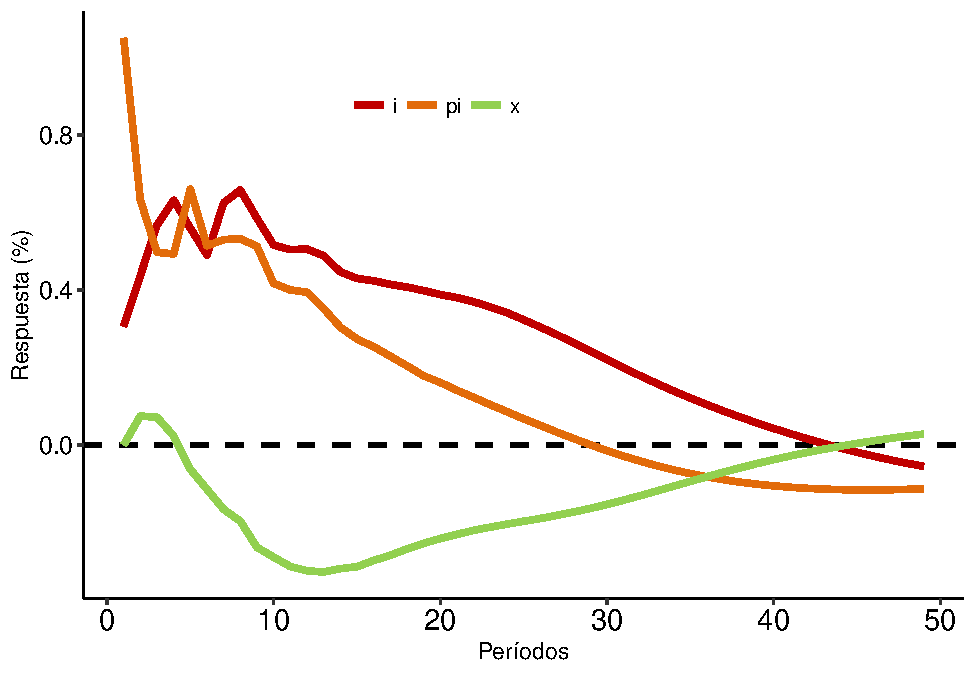
\includegraphics{01-conceptos_files/figure-latex/unnamed-chunk-5-1.pdf}

Finalmente, podemos observar la descomposición de la varianza de la variable \(\pi\):

\begin{Shaded}
\begin{Highlighting}[]
\NormalTok{fevd.p }\OtherTok{\textless{}{-}} \FunctionTok{fevd}\NormalTok{(Sims\_mdl, }\AttributeTok{n.ahead =} \DecValTok{48}\NormalTok{)}\SpecialCharTok{$}\NormalTok{p}
\NormalTok{RESULTADO}\OtherTok{\textless{}{-}}\FunctionTok{as.data.frame}\NormalTok{(fevd.p)}
\NormalTok{PERIODO}\OtherTok{\textless{}{-}}\FunctionTok{seq}\NormalTok{(}\DecValTok{1}\NormalTok{,}\DecValTok{48}\NormalTok{,}\DecValTok{1}\NormalTok{)}
\NormalTok{RESULTADO }\OtherTok{\textless{}{-}}\FunctionTok{cbind}\NormalTok{(RESULTADO,PERIODO)}
\NormalTok{BASE\_LONG }\OtherTok{\textless{}{-}} \FunctionTok{gather}\NormalTok{(RESULTADO, }\AttributeTok{key=}\StringTok{"measure"}\NormalTok{, }\AttributeTok{value=}\StringTok{"value"}\NormalTok{,}
                    \FunctionTok{c}\NormalTok{(}\StringTok{"x"}\NormalTok{, }\StringTok{"pi"}\NormalTok{, }\StringTok{"i"}\NormalTok{))}
\NormalTok{paleta}\OtherTok{\textless{}{-}}\FunctionTok{c}\NormalTok{(}\StringTok{"\#66C2A5"}\NormalTok{,}\StringTok{"\#8DA0CB"}\NormalTok{, }\StringTok{"\#E78AC3"}\NormalTok{)}
\NormalTok{Z}\OtherTok{\textless{}{-}}\FunctionTok{ggplot}\NormalTok{(BASE\_LONG, }\FunctionTok{aes}\NormalTok{(}\AttributeTok{x=}\NormalTok{PERIODO, }\AttributeTok{y=}\NormalTok{value, }\AttributeTok{fill=}\NormalTok{measure))}\SpecialCharTok{+}
  \FunctionTok{geom\_bar}\NormalTok{(}\AttributeTok{stat=}\StringTok{\textquotesingle{}identity\textquotesingle{}}\NormalTok{)}\SpecialCharTok{+}\FunctionTok{labs}\NormalTok{(}\AttributeTok{y=}\StringTok{""}\NormalTok{, }\AttributeTok{x=}\StringTok{""}\NormalTok{)}\SpecialCharTok{+}
  \FunctionTok{scale\_fill\_manual}\NormalTok{(}\AttributeTok{values =}\NormalTok{ paleta)}
\NormalTok{Z}\OtherTok{\textless{}{-}}\NormalTok{Z}\SpecialCharTok{+}\FunctionTok{labs}\NormalTok{(}\AttributeTok{y=}\StringTok{"Varianza (\%)"}\NormalTok{,}
          \AttributeTok{x=}\StringTok{"Períodos"}\NormalTok{)}
\NormalTok{Z}\OtherTok{\textless{}{-}}\NormalTok{Z}\SpecialCharTok{+}\FunctionTok{theme\_classic}\NormalTok{()}\SpecialCharTok{+}\FunctionTok{theme}\NormalTok{(}
  \AttributeTok{axis.line.x        =} \FunctionTok{element\_line}\NormalTok{(}\AttributeTok{colour =} \StringTok{"black"}\NormalTok{, }\AttributeTok{size =} \FloatTok{0.5}\NormalTok{),}
  \AttributeTok{axis.line.y.left   =} \FunctionTok{element\_line}\NormalTok{(}\AttributeTok{colour =} \StringTok{"black"}\NormalTok{, }\AttributeTok{size =} \FloatTok{0.5}\NormalTok{),}
  \AttributeTok{axis.line.y.right  =} \FunctionTok{element\_line}\NormalTok{(}\AttributeTok{colour =} \StringTok{"black"}\NormalTok{, }\AttributeTok{size =} \FloatTok{0.5}\NormalTok{),}
  \AttributeTok{axis.text.x        =} \FunctionTok{element\_text}\NormalTok{( }\AttributeTok{color =} \StringTok{"black"}\NormalTok{, }\AttributeTok{size =} \DecValTok{12}\NormalTok{),}
  \AttributeTok{axis.text.y        =} \FunctionTok{element\_text}\NormalTok{( }\AttributeTok{color =} \StringTok{"black"}\NormalTok{, }\AttributeTok{size =} \DecValTok{12}\NormalTok{),}
  \AttributeTok{panel.grid.major.y =} \FunctionTok{element\_line}\NormalTok{(}\AttributeTok{size =} \FloatTok{0.5}\NormalTok{,}
                                    \AttributeTok{linetype =} \StringTok{\textquotesingle{}solid\textquotesingle{}}\NormalTok{, }\AttributeTok{colour =} \StringTok{"\#EAEAF2"}\NormalTok{),}
  \AttributeTok{panel.grid.major.x =} \FunctionTok{element\_line}\NormalTok{(}\AttributeTok{size =} \FloatTok{0.5}\NormalTok{,}
                                    \AttributeTok{linetype =} \StringTok{\textquotesingle{}solid\textquotesingle{}}\NormalTok{, }\AttributeTok{colour =} \StringTok{"\#EAEAF2"}\NormalTok{),}
  \AttributeTok{panel.grid.minor.x =} \FunctionTok{element\_line}\NormalTok{(}\AttributeTok{size =} \FloatTok{0.5}\NormalTok{,}
                                    \AttributeTok{linetype =} \StringTok{\textquotesingle{}solid\textquotesingle{}}\NormalTok{, }\AttributeTok{colour =} \StringTok{"\#EAEAF2"}\NormalTok{),}
  \AttributeTok{panel.grid.minor.y =} \FunctionTok{element\_line}\NormalTok{(}\AttributeTok{size =} \FloatTok{0.5}\NormalTok{,}
                                    \AttributeTok{linetype =} \StringTok{\textquotesingle{}solid\textquotesingle{}}\NormalTok{, }\AttributeTok{colour =} \StringTok{"\#EAEAF2"}\NormalTok{),}
  \AttributeTok{strip.background.x =} \FunctionTok{element\_rect}\NormalTok{(}\AttributeTok{colour=}\StringTok{"black"}\NormalTok{, }\AttributeTok{fill=}\StringTok{"gray"}\NormalTok{),}
  \AttributeTok{strip.text.x       =} \FunctionTok{element\_text}\NormalTok{(}\AttributeTok{size =} \DecValTok{20}\NormalTok{, }\AttributeTok{color =} \StringTok{"black"}\NormalTok{, }\AttributeTok{face =} \StringTok{"bold.italic"}\NormalTok{),}
  \AttributeTok{legend.title =} \FunctionTok{element\_blank}\NormalTok{(),}
  \AttributeTok{legend.text  =} \FunctionTok{element\_text}\NormalTok{(}\AttributeTok{size=}\DecValTok{18}\NormalTok{),}
  \AttributeTok{legend.position=}\StringTok{"bottom"}\NormalTok{,}
  \AttributeTok{legend.spacing.x =} \FunctionTok{unit}\NormalTok{(}\FloatTok{0.20}\NormalTok{, }\StringTok{\textquotesingle{}cm\textquotesingle{}}\NormalTok{),}
  \AttributeTok{legend.margin=}\FunctionTok{margin}\NormalTok{(),}
  \AttributeTok{legend.background =} \FunctionTok{element\_rect}\NormalTok{(}\AttributeTok{fill =} \StringTok{"white"}\NormalTok{, }\AttributeTok{colour =} \StringTok{"transparent"}\NormalTok{,}
                                   \AttributeTok{color =} \StringTok{"white"}\NormalTok{, }\AttributeTok{inherit.blank =} \ConstantTok{FALSE}\NormalTok{)}
\NormalTok{)}\SpecialCharTok{+}\FunctionTok{guides}\NormalTok{(}\AttributeTok{color =} \FunctionTok{guide\_legend}\NormalTok{(}\AttributeTok{nrow =} \DecValTok{1}\NormalTok{))}
\NormalTok{Z}
\end{Highlighting}
\end{Shaded}

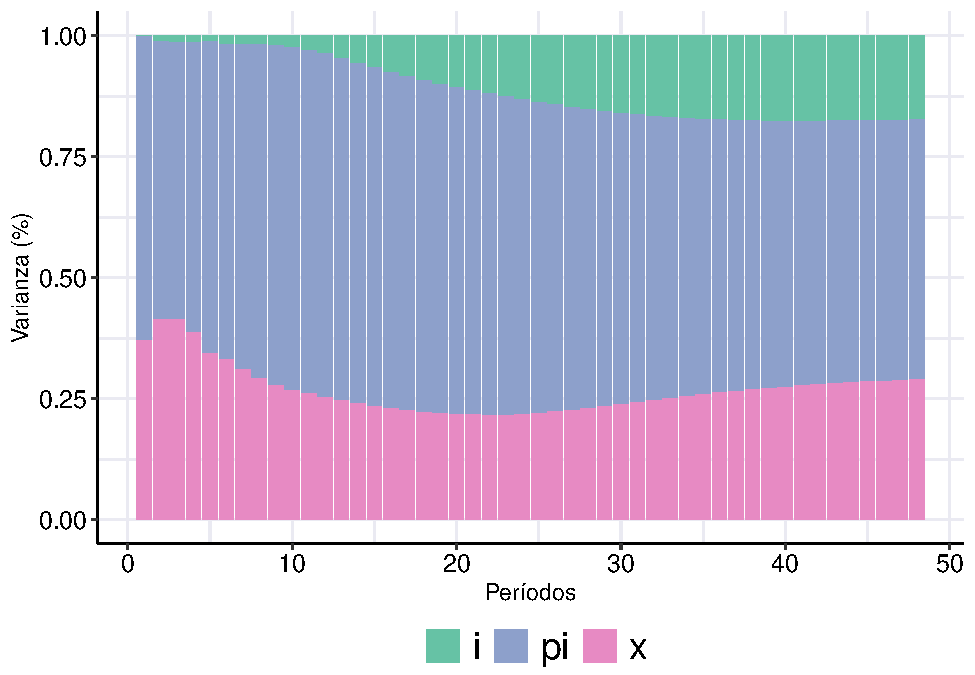
\includegraphics{01-conceptos_files/figure-latex/unnamed-chunk-6-1.pdf}

A continuación se replicará los resultados obtenidos por \citet{Herwartz2016}, específicamente se estimaran los shocks estructurales a través de la metodología de cambios en volatilidades. Ello se logra a través de la función \emph{id.cv()} dentro del cual hay que indicarle la fecha a partir de la cual se dio ese cambio estructural.

\citet{Herwartz2016} argumentan que el punto de quiebra se dio en el tercer trimestre de 1979 donde aconteció un cambio en la política de la Reserva Federal que redujo la volatilidad de las variables macroeconómicas (ver \citet{Stock2003})

Lo anterior es posible visualizarlo.
Un primer paso es visualizar cada una de las series.

\begin{Shaded}
\begin{Highlighting}[]
\FunctionTok{autoplot}\NormalTok{(usa, }\AttributeTok{facets =}\NormalTok{ T) }\SpecialCharTok{+} \FunctionTok{theme\_bw}\NormalTok{() }\SpecialCharTok{+} \FunctionTok{ylab}\NormalTok{(}\StringTok{\textquotesingle{}Evolución de series de USA\textquotesingle{}}\NormalTok{)}
\end{Highlighting}
\end{Shaded}

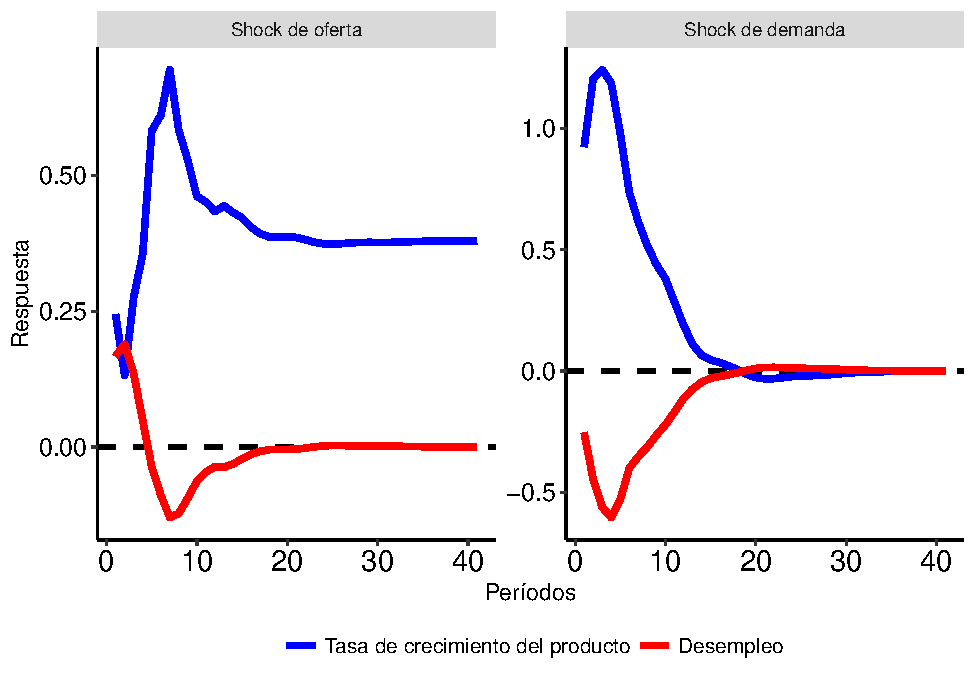
\includegraphics{01-conceptos_files/figure-latex/unnamed-chunk-7-1.pdf}

Con base en el objeto VAR podemos estimar su forma estructural con la función \emph{id.cv()} la cual introduce el \emph{cambio en la varianza} que se observa en las series, sin embargo la aplicación de esta función requiere específicar el argumento \emph{SB} en formato \emph{ts}:

\begin{Shaded}
\begin{Highlighting}[]
\NormalTok{usa.cv }\OtherTok{\textless{}{-}} \FunctionTok{id.cv}\NormalTok{(plain.var, }\AttributeTok{SB =} \FunctionTok{c}\NormalTok{(}\DecValTok{1979}\NormalTok{, }\DecValTok{3}\NormalTok{))}
\FunctionTok{summary}\NormalTok{(usa.cv)}
\end{Highlighting}
\end{Shaded}

\begin{verbatim}
## 
## Identification Results
## ---------------------- 
## 
## Method: Changes in Volatility
## Sample size: 169
## Log-Likelihood: -564.2994
## AIC: 1268.599
## Structural Break: At Observation Number 59 during 1979 Q3
## Number of GLS estimations: 22
## Number of Restrictions: 0
## 
## Estimated unconditional Heteroscedasticity Matrix (Lambda):
##         [,1]     [,2]     [,3]
## x  0.3925906 0.000000 0.000000
## pi 0.0000000 0.191641 0.000000
## i  0.0000000 0.000000 1.244348
## 
## Standard Errors of Lambda:
##         [,1]       [,2]      [,3]
## x  0.0926582 0.00000000 0.0000000
## pi 0.0000000 0.04527264 0.0000000
## i  0.0000000 0.00000000 0.2935572
## 
## Estimated B Matrix (unique decomposition of the covariance matrix): 
##           [,1]       [,2]      [,3]
## x   0.61193300 -0.5931964 0.2241237
## pi  0.75559400  1.2987520 0.1131134
## i  -0.02899916  0.1572953 0.7084709
## 
## Standard Errors of B:
##         [,1]      [,2]       [,3]
## x  0.1330924 0.1955350 0.07101215
## pi 0.2498465 0.2600375 0.09960246
## i  0.1559672 0.1213446 0.07004431
## 
## Identification Wald Test of equal Eigenvalues:
## [1] 1.2443485 0.3925906 0.1916410
##                              Test statistic dof p-value  
## lambda_ 1 =lambda_2                  5.3828   2 0.06779 .
## lambda_ 1 =lambda_2=lambda_3        15.0586   5 0.01011 *
## lambda_ 2 =lambda_3                  2.1465   2 0.34189  
## ---
## Signif. codes:  0 '***' 0.001 '**' 0.01 '*' 0.05 '.' 0.1 ' ' 1
\end{verbatim}

Si el VAR puede ser escrito con matrices y como un sistema de media móviles (como se vió anteriormente) de la siguiente forma:

\begin{align}
x_{t}&=B^{*}(L)\epsilon_{t},\;\;B^{*}(0)=I,\;\;E(w_{t}w_{t}^{'})=\Sigma_w 
\end{align}

Los resultados muestran la matriz de covarianza estimada \(\hat{B^{*}}\), la matriz de cambio en la convarianza estiamda \(\hat{\lambda}\).

Es de notar que el orden de las columnas en \(\hat{B^{*}}\) es arbitrario. Lo importante es que ese ordenamiento se haga teniendo un sentido económico.

\citet{Herwartz2016} con base en los resultados de la matriz \(\hat{B^{*}}\) hace un ordenamiento de acuerdo con el patrón de los signos. Ello indica que la columna 3 obdece a un shock de demanda, la columna 2 a un shock de oferta y la columna 1 a un shock de política monetaria. El siguiente código ordena las columnas de esa misma manera.

\begin{Shaded}
\begin{Highlighting}[]
\NormalTok{usa.cv}\SpecialCharTok{$}\NormalTok{B }\OtherTok{\textless{}{-}}\NormalTok{ usa.cv}\SpecialCharTok{$}\NormalTok{B[, }\FunctionTok{c}\NormalTok{(}\DecValTok{3}\NormalTok{, }\DecValTok{2}\NormalTok{, }\DecValTok{1}\NormalTok{)]}
\NormalTok{usa.cv}\SpecialCharTok{$}\NormalTok{B[,}\DecValTok{3}\NormalTok{] }\OtherTok{\textless{}{-}}\NormalTok{ usa.cv}\SpecialCharTok{$}\NormalTok{B[, }\DecValTok{3}\NormalTok{] }\SpecialCharTok{*}\NormalTok{ (}\SpecialCharTok{{-}}\DecValTok{1}\NormalTok{)}
\NormalTok{usa.cv}\SpecialCharTok{$}\NormalTok{B\_SE }\OtherTok{\textless{}{-}}\NormalTok{ usa.cv}\SpecialCharTok{$}\NormalTok{B\_SE[, }\FunctionTok{c}\NormalTok{(}\DecValTok{3}\NormalTok{, }\DecValTok{2}\NormalTok{, }\DecValTok{1}\NormalTok{)]}
\NormalTok{usa.cv}\SpecialCharTok{$}\NormalTok{Lambda }\OtherTok{\textless{}{-}} \FunctionTok{diag}\NormalTok{(}\FunctionTok{diag}\NormalTok{(usa.cv}\SpecialCharTok{$}\NormalTok{Lambda)[}\FunctionTok{c}\NormalTok{(}\DecValTok{3}\NormalTok{, }\DecValTok{2}\NormalTok{, }\DecValTok{1}\NormalTok{)])}
\NormalTok{usa.cv}\SpecialCharTok{$}\NormalTok{Lambda\_SE }\OtherTok{\textless{}{-}} \FunctionTok{diag}\NormalTok{(}\FunctionTok{diag}\NormalTok{(usa.cv}\SpecialCharTok{$}\NormalTok{Lambda\_SE)[}\FunctionTok{c}\NormalTok{(}\DecValTok{3}\NormalTok{, }\DecValTok{2}\NormalTok{, }\DecValTok{1}\NormalTok{)])}
\FunctionTok{round}\NormalTok{(usa.cv}\SpecialCharTok{$}\NormalTok{B, }\DecValTok{3}\NormalTok{)}
\end{Highlighting}
\end{Shaded}

\begin{verbatim}
##     [,1]   [,2]   [,3]
## x  0.224 -0.593 -0.612
## pi 0.113  1.299 -0.756
## i  0.708  0.157  0.029
\end{verbatim}

\citet{Herwartz2016} interpretan el efecto de la primera columna de la matriz \(\hat{B^{*}}\) como un shock de demanda. La segunda y tercera columna representa un shock de oferta y la tercera un shock de política monetaria.

\begin{Shaded}
\begin{Highlighting}[]
\FunctionTok{round}\NormalTok{(usa.cv}\SpecialCharTok{$}\NormalTok{Lambda, }\DecValTok{3}\NormalTok{)}
\end{Highlighting}
\end{Shaded}

\begin{verbatim}
##       [,1]  [,2]  [,3]
## [1,] 1.244 0.000 0.000
## [2,] 0.000 0.192 0.000
## [3,] 0.000 0.000 0.393
\end{verbatim}

En cambio la matriz \(\hat{\lambda}\) representa la varianza de los shocks estructurales en un segundo regimén, esto es posterior al quiebre estructural. Los autores interpretan a partir de la diagonal de \(\hat{\lambda}\) que los shocks de oferta y política monetaria tiene baja varianza en comparación a los shocks de demanda.

Los autores comparan estos resultados con los obtenidos por \citet{Sims80} utilizando la descomposición de la matriz de covarianza (\(\hat{B}\)) como una matriz triangular inferior. La función \emph{id.cv()} permite
probar tales restricciones configurando para ello una matriz triangular inferior como se describe en el código siguiente.

\begin{Shaded}
\begin{Highlighting}[]
\NormalTok{restMat }\OtherTok{\textless{}{-}} \FunctionTok{matrix}\NormalTok{(}\FunctionTok{rep}\NormalTok{(}\ConstantTok{NA}\NormalTok{, }\DecValTok{9}\NormalTok{), }\AttributeTok{ncol =} \DecValTok{3}\NormalTok{)}
\NormalTok{restMat[}\DecValTok{1}\NormalTok{, }\FunctionTok{c}\NormalTok{(}\DecValTok{2}\NormalTok{, }\DecValTok{3}\NormalTok{)] }\OtherTok{\textless{}{-}} \DecValTok{0}
\NormalTok{restMat[}\DecValTok{2}\NormalTok{, }\DecValTok{3}\NormalTok{] }\OtherTok{\textless{}{-}} \DecValTok{0}
\NormalTok{restMat}
\end{Highlighting}
\end{Shaded}

\begin{verbatim}
##      [,1] [,2] [,3]
## [1,]   NA    0    0
## [2,]   NA   NA    0
## [3,]   NA   NA   NA
\end{verbatim}

\begin{Shaded}
\begin{Highlighting}[]
\NormalTok{restricted.model }\OtherTok{\textless{}{-}} \FunctionTok{id.cv}\NormalTok{(plain.var, }\AttributeTok{SB =} \FunctionTok{c}\NormalTok{(}\DecValTok{1979}\NormalTok{, }\DecValTok{3}\NormalTok{),}\AttributeTok{restriction\_matrix =}\NormalTok{ restMat)}
\FunctionTok{summary}\NormalTok{(restricted.model)}
\end{Highlighting}
\end{Shaded}

\begin{verbatim}
## 
## Identification Results
## ---------------------- 
## 
## Method: Changes in Volatility
## Sample size: 169
## Log-Likelihood: -568.6664
## AIC: 1277.333
## Structural Break: At Observation Number 59 during 1979 Q3
## Number of GLS estimations: 23
## Number of Restrictions: 3
## 
## Estimated unconditional Heteroscedasticity Matrix (Lambda):
##         [,1]      [,2]      [,3]
## x  0.3501948 0.0000000 0.0000000
## pi 0.0000000 0.2346854 0.0000000
## i  0.0000000 0.0000000 0.9420116
## 
## Standard Errors of Lambda:
##          [,1]       [,2]     [,3]
## x  0.08266738 0.00000000 0.000000
## pi 0.00000000 0.05616318 0.000000
## i  0.00000000 0.00000000 0.227189
## 
## Estimated B Matrix (unique decomposition of the covariance matrix): 
##          [,1]      [,2]      [,3]
## x  0.87988465 0.0000000 0.0000000
## pi 0.08137972 1.5306503 0.0000000
## i  0.31518384 0.2606745 0.7378484
## 
## Standard Errors of B:
##          [,1]       [,2]       [,3]
## x  0.08638851 0.00000000 0.00000000
## pi 0.10334026 0.15169565 0.00000000
## i  0.08527441 0.08620187 0.07354585
## 
## Identification Wald Test of equal Eigenvalues:
## [1] 0.9420116 0.3501948 0.2346854
##                              Test statistic dof p-value
## lambda_ 1 =lambda_2                 4.04784   2  0.1321
## lambda_ 1 =lambda_2=lambda_3        9.15413   5  0.1031
## lambda_ 2 =lambda_3                 0.68408   2  0.7103
## 
## Likelihood Ratio Test: 
##  Test statistic p-value  
##           8.734   0.033 *
## ---
## Signif. codes:  0 '***' 0.001 '**' 0.01 '*' 0.05 '.' 0.1 ' ' 1
\end{verbatim}

Si partimos que los shocks structurales fueron identificados con la metodología de cambio en la matriz de covarianza, cualquier restricción impuesta sobre \(B\) hace que el modelo esté sobre identificado y ello es posible probarse.

En resumen el \emph{likelihood ratio test} indica que bajo la \(H_{0}\)
que \(B\) la matriz triangular (baja la cual impactan los shocks structurales) es rechazada al \(5\%\) de nivel de significancia.

\citet{Herwartz2016} argumentan que la identificación de valores iguales a cero para lograr una matriz trinagular inferior es algo contra intuitivo desde el punto de vista económico; por tanto un modelo sin restricciones debería ser preferido.

El siguiente paso es calcular la función impulso respuesta (IFR) con un intervalo de confianza obtenido a partir del método ``boostrap''. A partir de la IFR es posible investigar los efectos futuros de los shocks estructurales etiquetados como ``económicos'' sobre las variables
incluidas en el modelo. De hecho de acuerdo a \citet{Herwartz18} aplicar la metodología "boostrap permite evaluar la significancia en los signos que se hacen patentes en la matriz \(\hat{B}\).

Para aplicar lo anterior, definimos una lista con los signos que representan nuestras restricciones tanto para los shocks de demanda, oferta y política monetaria.

\begin{Shaded}
\begin{Highlighting}[]
\NormalTok{signrest }\OtherTok{\textless{}{-}} \FunctionTok{list}\NormalTok{(}\AttributeTok{demand =} \FunctionTok{c}\NormalTok{(}\DecValTok{1}\NormalTok{, }\DecValTok{1}\NormalTok{, }\DecValTok{1}\NormalTok{), }\AttributeTok{supply =} \FunctionTok{c}\NormalTok{(}\SpecialCharTok{{-}}\DecValTok{1}\NormalTok{, }\DecValTok{1}\NormalTok{, }\DecValTok{1}\NormalTok{), }\AttributeTok{monetary\_policy =} \FunctionTok{c}\NormalTok{(}\SpecialCharTok{{-}}\DecValTok{1}\NormalTok{, }\SpecialCharTok{{-}}\DecValTok{1}\NormalTok{, }\DecValTok{1}\NormalTok{))}
\end{Highlighting}
\end{Shaded}

Notar que el horizonte de tiempo para el IFR tiene que ser determinado de antemano usando el argumento n.ahead.

\begin{Shaded}
\begin{Highlighting}[]
\NormalTok{cores }\OtherTok{\textless{}{-}}\NormalTok{ parallel}\SpecialCharTok{::}\FunctionTok{detectCores}\NormalTok{() }\SpecialCharTok{{-}} \DecValTok{1}
\FunctionTok{set.seed}\NormalTok{(}\DecValTok{231}\NormalTok{)}
\NormalTok{usa.cv.boot }\OtherTok{\textless{}{-}} \FunctionTok{wild.boot}\NormalTok{(usa.cv, }\AttributeTok{design =} \StringTok{"fixed"}\NormalTok{,}\AttributeTok{distr =} \StringTok{"rademacher"}\NormalTok{, }\AttributeTok{nboot =} \DecValTok{1000}\NormalTok{, }\AttributeTok{n.ahead =} \DecValTok{15}\NormalTok{,}\AttributeTok{nc =}\NormalTok{ cores, }\AttributeTok{signrest =}\NormalTok{ signrest)}
\FunctionTok{summary}\NormalTok{(usa.cv.boot)}
\end{Highlighting}
\end{Shaded}

\begin{verbatim}
## 
## Bootstrap Results
## ----------------- 
## 
## Method: Wild bootstrap
## Bootstrap iterations: 1000
## Distribution used: rademacher
## Design: fixed
## 
## Point estimates: 
##         [,1]       [,2]        [,3]
## x  0.2241237 -0.5931964 -0.61193300
## pi 0.1131134  1.2987520 -0.75559400
## i  0.7084709  0.1572953  0.02899916
## 
## Bootstrap means: 
##          [,1]       [,2]       [,3]
## x  0.09580740 -0.5030485 -0.6303868
## pi 0.09639712  1.1310905 -0.7720157
## i  0.70100321  0.0364798 -0.1675659
## 
## Bootstrap standard errors: 
##          [,1]      [,2]      [,3]
## x  0.14143383 0.3077349 0.2494872
## pi 0.17500155 0.4556690 0.5925734
## i  0.07511879 0.2273595 0.2178134
## 
## Identified sign patterns: 
## =========================
## Specified sign pattern: 
## 
##    demand supply monetary_policy
## x       1     -1              -1
## pi      1      1              -1
## i       1      1               1
## 
## Unique occurrence of single shocks according to sign pattern: 
## demand : 65.5 % 
## supply : 66 % 
## monetary_policy : 28.4 % 
## 
## Joint occurrence of specified shocks: 12.7 %
\end{verbatim}

Enseguida, graficamos para cada variable y shocks su IFR.

\begin{Shaded}
\begin{Highlighting}[]
\FunctionTok{plot}\NormalTok{(usa.cv.boot, }\AttributeTok{lowerq =} \FloatTok{0.16}\NormalTok{, }\AttributeTok{upperq =} \FloatTok{0.84}\NormalTok{)}
\end{Highlighting}
\end{Shaded}

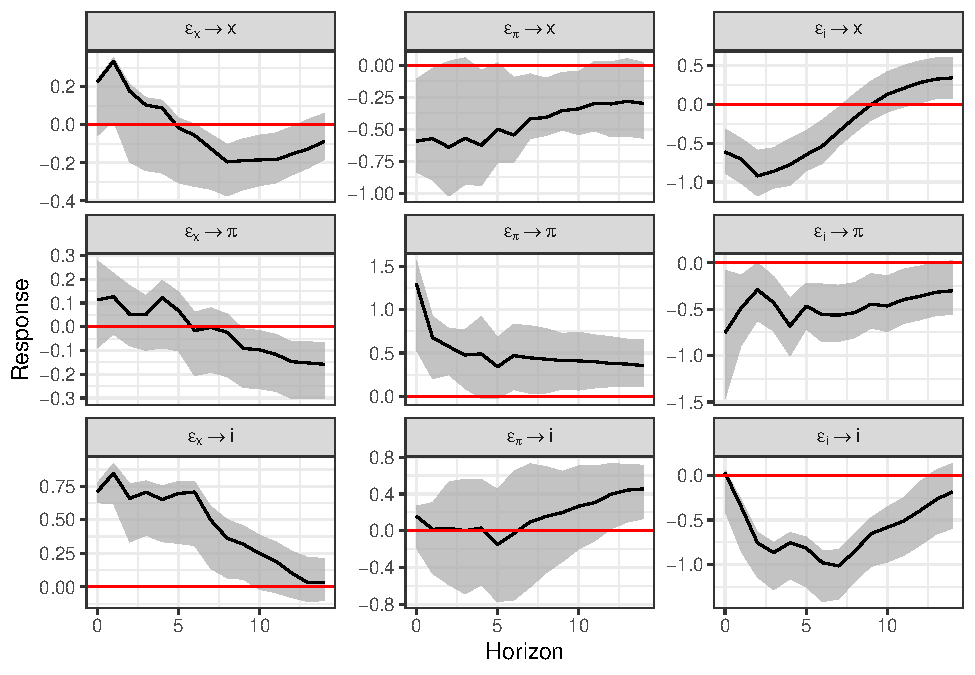
\includegraphics{01-conceptos_files/figure-latex/unnamed-chunk-15-1.pdf}

El resumen el resultado revela que solo el 12.7\% de todas las estimaciones hechas a través de bootstrap están en línea con lo que la teoría económica nos sugeriría que debería corresponder con los patrones de los signos motivados en forma conjunta.

El patrón de signos del shock de política monetaria aparece en solo el 28,4\% de todas los experimentos.

En tanto, la metodología bootstrap indica que el tercer choque está más en línea con el patrón de signos del choque de demanda. Este resultado es plausible observando que la estimación puntual en la esquina inferior derecha es cercana a cero y, por lo tanto, carece de un efecto significativamente positivo sobre la tasa de interés.

La Figura anterior muestra las funciones de impulso-respuesta de choques normalizados con varianza unitaria en el primer régimen.

\citet{Herwartz2016} argumentan que la reacción negativa de la tasa de interés a un shock de política monetaria después del período inicial es inverosímil, y pone en duda que este shock se interpreta como uno de política monetaria. Los resultados del bootstrap apoyan la argumentación de los autores con
con respecto al etiquetado de choque.

Además, podemos calcular la descomposición de la varianza del error de pronóstico para investigar la contribución de cada perturbación al error cuadrático medio de predicción de las variables. El método \emph{fevd()}
crea un objeto para la inspección visual de la descomposición de la varianza del error.

\begin{Shaded}
\begin{Highlighting}[]
\NormalTok{fev.cv }\OtherTok{\textless{}{-}} \FunctionTok{fevd}\NormalTok{(usa.cv, }\AttributeTok{n.ahead =} \DecValTok{48}\NormalTok{)}
\FunctionTok{plot}\NormalTok{(fev.cv)}
\end{Highlighting}
\end{Shaded}

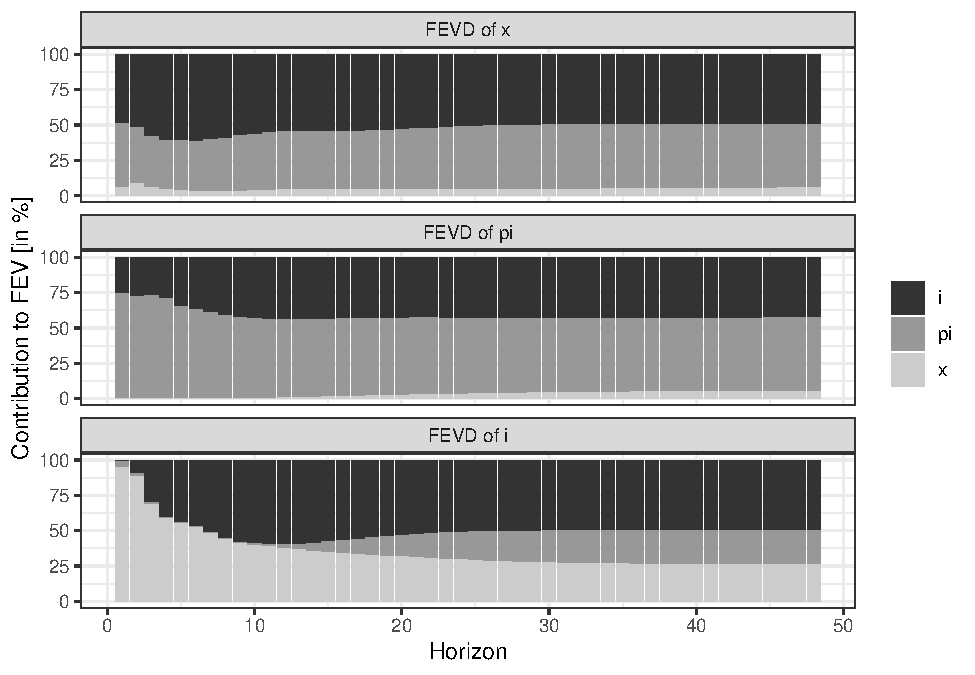
\includegraphics{01-conceptos_files/figure-latex/unnamed-chunk-16-1.pdf}

De acuerdo a la anterior figura es evidente que el shock de política monetaria explica más del 50\% del error cuadrático medio de predicción de la brecha del producto, mientras que el choque de demanda representa constantemente solo alrededor del 5\% de la media de predicción
error al cuadrado.

Además, el shock de demanda contribuye casi al 100\% del error de pronóstico
varianza de las tasas de interés.

Por lo tanto, las descomposiciones del error de pronóstico apuntan a un
etiquetado de los choques diferente del desarrollado anteriormente sobre la base de patrones de signos de \(\hat{B^{*}}\). Además, confirman la conclusión de \citet{Herwartz2016} de que el modelo enpirico no logra identificar un shock de política monetaria de acuerdo con sus patrones basados en la teoría económica.

\hypertarget{bla-bla}{%
\section{BLA Bla}\label{bla-bla}}

La estructura del modelo determina el orden de prelación de cada una de las variables y las restricciones de corto plazo.
El vector está dado por X={[}y, \(\pi\), i, NPL, L, e{]} y se establece un SVAR de la forma \(AX=X_{-1}+u\), en el que A contiene las restricciones y con el cual se identifica los shocks.
Los datos utilizados tienen la siguiente características:\}

\begin{eqnarray}
AX&=\begin{bmatrix}
1 & 0 & 1 & 0 & 0 & 0  \\
1 & 1 & 0 & 0 & 0 & 0 \\
0 & 1 & 1 & 1 & 0 & 0 \\
0 & 0 & 0 & 1 & 0 & 0 \\
1 & 1 & 1 & 1 & 1 & 0 \\
1 & 1 & 1 & 1 & 1 & 1 \end{bmatrix}
\begin{bmatrix}
y \\
\pi \\
i\\
NPL\\
L\\
e\end{bmatrix}
\end{eqnarray}

  \bibliography{book.bib,packages.bib}

\end{document}
